\documentclass[hidelinks]{report}

% Comment out if this isn't the draft!
% \usepackage[firstpageonly]{draftwatermark}

\usepackage[T1]{fontenc}

\usepackage{unicode-math}
\setmainfont{Gentium Basic}
\setmonofont{Fantasque Sans Mono}

\usepackage{microtype}

\usepackage{xcolor}
\definecolor{Thesis}{HTML}{297544}
\definecolor{Thesis2}{HTML}{65d66f}
\definecolor{BG}{HTML}{ffffff}
\definecolor{FG}{HTML}{000000}

% Secret dark theme
% \definecolor{Thesis}{HTML}{65d66f}
% \definecolor{Thesis2}{HTML}{297544}
% \definecolor{FG}{HTML}{f2f2f2}
% \definecolor{BG}{HTML}{0b1210}

\usepackage{listings}
\lstset{frame=single,basicstyle={\footnotesize\ttfamily},linewidth=0.8\textwidth}

\usepackage{graphicx}
\graphicspath{{files/}}

\usepackage[allbordercolors=Thesis]{hyperref}
\newcommand*{\requirementautorefname}{Requirement}

\usepackage{tikz}
\usetikzlibrary{shapes.geometric, positioning}
% tikz style
\tikzstyle{startstop} = [rectangle, rounded corners, minimum width=2cm, minimum height=1cm,text centered, draw=black]
\tikzstyle{io} = [trapezium, trapezium left angle=70, trapezium right angle=110, minimum width=2cm, minimum height=0.75cm, text centered, draw=black]
\tikzstyle{process} = [rectangle, minimum width=2cm, minimum height=1cm, text centered, draw=black]
\tikzstyle{decision} = [diamond, minimum width=2cm, minimum height=1cm, text centered, draw=black]

\usepackage{array}
\usepackage{booktabs}

\usepackage[labelfont=bf]{caption}

\usepackage[a4paper]{geometry}
\usepackage{parskip}

\newcommand{\unchapter}[2]{
    \setcounter{chapter}{#1}
    \setcounter{section}{0}
    \chapter*{#2}
    \addcontentsline{toc}{chapter}{#2}
}

\usepackage{setspace}
\onehalfspacing

\usepackage{multicol}

\newtheorem{requirement}{Requirement}

\color{FG}
\pagecolor{BG}

\begin{document}

\begin{titlepage}

\vspace*{\fill}

\begin{center}
    
\includegraphics{unsw}
\end{center}

\vspace{0.5cm}

\begin{center}
    \Large{}School of Computer Science and Engineering\\
    Faculty of Engineering\\
    The University of New South Wales
\end{center}

\vspace{1cm}

\begin{center}
    \Huge \textbf{A Testing Tool for Introductory Programming Courses}
\end{center}

\vspace{0.35cm}

\begin{center}
    \Large{}By Kyu-Sang Kim\\
    {\normalsize z5208931}
    
    \vspace{0.25cm}
    
    Supervised by Andrew Taylor (UNSW)\\
    Assessed by John Shepherd (UNSW)
\end{center}

\vspace{0.75cm}

\begin{center}
    \textbf{Thesis A Report} --- Term 1, 2022\\
    Submitted \textit{April 2022}
    
    \vspace{0.1cm}
    
    Thesis submitted as a requirement for the degree of\\
    Bachelor of Engineering in Software Engineering (Honours)
\end{center}

\vspace*{\fill}

\end{titlepage}

\begin{abstract}
\textit{Automated code testing tools} are valuable to course staff in the administration of \textit{practical coding assessments} to students. In this thesis, we will evaluate the architecture and implementations of \textit{automated code testing tools} such as \textit{autotest}, and develop a new software package with the proper \textit{technical debt} management procedures. Thus, this thesis aims to design and implement a \textit{automated code testing tool} that replaces the existing \textit{autotest} at UNSW introductory programming courses and has measures implemented to minimise technical debt into the long term.
\end{abstract}

\unchapter{0}{Acknowledgements}

I would like to thank Andrew Taylor and John Shepherd for their guidance as supervisor and assessor for this project respectively. I would also like to thank the numerous UNSW Computer Science and Engineering school course administrators who have taken interest in the project by providing their thoughts and ideas: Shrey Somaiya, Zac Kologlu and Tom Kunc.

Finally, I would like to thank my family and friends for all their support during both my degree and this thesis. 

\unchapter{0}{Abbreviations}

\textbf{UNSW} The University of New South Wales\\
\textbf{CSE} Computer Science and Engineering School\\
\textbf{pip} PIP Installs Packages - de facto and recommended package installer for Python\\
\textbf{MVP} Minimal Viable Product\\

\tableofcontents

\listoffigures

\listoftables

\unchapter{1}{Introduction}

\section{Motivation}
\subsection{Student Enrolments \& Practical Coding Assessments}
In recent years, student enrolments in introductory programming courses at UNSW have increased at an extraordinary rate. Despite the increase in students, course staff must still continue to deliver the best learning experience, fulfil course outcomes and provide a numerical ``mark" to students upon course completion.

\begin{table}[h]
	\centering
	\begin{tabular}{llllll}
		\toprule
		Course/Year & 2017 & 2018 & 2019 & 2020 & 2021 \\
		\midrule
		COMP1511       & 1351 & 1655 & 1874 & 1905 & 2381 \\
		COMP1521       & 715 & 1136 & 1352 & 1417 & 1633 \\
		COMP2521       & 378 & 1019 & 1389 & 1445 & 1551 \\
		\bottomrule
	\end{tabular}
	\caption{Course enrolments from UNSW Class Timetable (April 2022)}
	\label{tab:table1}
\end{table}

One approach taken by UNSW computing courses to assist in calculating a student's ``mark" are \textit{practical coding assessments}. They allow for students to demonstrate their knowledge and understanding of the course content which can then be assessed at a later time by course staff.

In order to support course staff in the administration of these \textit{practical coding assessments}, \textit{automated code testing tools} can be utilised to automatically determine the correctness of a student's submitted code to a given specification with minimal course staff intervention. The results of these tools can then be further processed to generate a grade for the student's code submission.

In some courses, these tools can also be made available to students by course staff to perform basic correctness checks on their code before submission. 
\clearpage

\subsection{Technical Debt}
In 1992, Ward Cunningham who first introduced the concept of \textit{technical debt} described it as how ``shipping first time code is like going into debt. A little debt speeds development so long as it is paid back promptly with a rewrite" \cite{TechnicalDebtConcept}.

Although the meaning of \textit{technical debt} varies on the context and each reader's interpretation, this thesis will assume \textit{technical debt} to be any component or aspect of a project that could be prescribed as a weakness or flaw by a reader or contributor. As an example, \textit{technical debt} could be observed as issues that hinder the ease of understanding and improvement of a project. 

\subsection{autotest}
\textit{autotest} is a Python-based \textit{automated code testing tool} written by Andrew Taylor which is an evolution of a earlier script by Mei Cheng Whale \cite{Autotest}. It was first introduced into the COMP2041 \textit{Software Construction: Techniques and Tools} course in the second semester of 2015 and has since become the standard for introductory programming courses at UNSW to automatically assess the correctness of code to a given specification.

Despite the gradual improvements and fixes made to \textit{autotest} since it's introduction, \textit{autotest} is plagued with \textit{design deficiencies} and non-trivial amounts of \textit{technical debt} which has affected the scalability of \textit{autotest} in response to increasing student numbers as well as complicate development of new features.

In particular, major shortcomings can be identified if we analyse the \textit{autotest} code to the framework defined within \textit{An Exploration of Technical Debt} \cite{TechnicalDebt}. A clear example is the Knowledge Distribution debt stemming from the ineffective documentation of \textit{autotest} which has hindered new users in their adoption of \textit{autotest} and confused code contributors on the inner-workings of the tool.

As a result of these findings, there were efforts undertaken in 2021 by the UNSW CSE community including Andrew Taylor to remediate major sources of technical debt from the \textit{autotest} tool in which some measures were successful. However, there exists issues such as the lack of documentation and software modernisation that has been seen as infeasible to fix without significant overhaul \cite{AutotestIssues}.

\section{Thesis Problem Statement}
\textit{Automated code testing tools} are valuable to course staff in the administration of \textit{practical coding assessments} to students. In this thesis, we will evaluate the architecture and implementations of \textit{automated code testing tools} such as \textit{autotest}, and develop a new software package with the proper \textit{technical debt} management procedures. Thus, this thesis aims to design and implement a \textit{automated code testing tool} that replaces the existing \textit{autotest} at UNSW introductory programming courses and has measures implemented to minimise technical debt into the long term.

\subsection{Thesis Structure}

Chapter 1 covers the motivations behind this thesis as well as the thesis problem statement.
Chapter 2 explains the background concepts that are relevant to understanding the later chapters of the thesis. Chapter 3 undertakes an evaluation and review of the existing works related to this thesis.
Chapter 4 declares design requirements/goals and proposes approaches that fulfil as many of the goals as possible before providing a justification for selecting one approach.
Chapter 5 outlines the preliminary work that has been completed so far outside of the thesis report and outlines the work plan for Thesis B and C.
Finally, Chapter 6 summarises the contents of this thesis report.

\unchapter{2}{Background}

First, it is important to explore what technical debt is and the various approaches to management, then it is possible to start looking at the concepts of how code marking is manually conducted and it's flaws at scale. This thesis will then evaluate the various approaches to automated code testing and how they can be applied to determine the correctness of code to a given specification.

\section{Management of Technical Debt}

Technical debt is inevitable in any project but implementing measures to understand, communicate and manage technical debt from the outset can make a huge difference in both the short- and long-term success of the project. One particular benefit is that contributors are able to make informed decisions which are aimed towards reducing the time and work required to understand and improve the project in both the short- and long-term \cite{TechnicalDebtManagement}.

To minimise sources of various technical debt in this thesis project, we will implement the following measures:
\begin{itemize}
	\item \textbf{Extensive project and code documentation} - Extensive project and code documentation will greatly assist a reader in understanding the usage and internals of project faster which will be useful for improvements in the future.
	\item \textbf{Project management tools} - Tools such as Github and Jira allow for the tracking of code and issues respectively to assist in communicating and management of technical debt between multiple project contributors to minimise confusion and allow each contributor to work independently.
	\item \textbf{Modular architectural design} - Approaching the project with a modular architectural design in mind will assist in long term development as decoupling dependencies between major components will make them easier to replace when upgraded.
	\item \textbf{Solution modernisation \& focus on feature extensibility} - Similar to modular architectural design, approaching the project with a focus in supporting easier solution modernisation and feature extensibility will reduce the need for a replacement of the entire project instead of targeted components.
	\item \textbf{Automated regression testing} - Automatic regression testing of code will assist in development by allowing contributors to create and improve features whilst enforcing an accepted baseline of program correctness. This ensures that minimal code errors which can also be considered technical debt is deployed for users of the project.
\end{itemize}

Successful implementation of the above measures will ensure that the project has minimal technical debt in both the development and post-release period.

\section{Code Testing \& Marking}

This thesis assumes that \textit{code marking} refers to the determination of whether provided code when executed conforms to some behaviour that is outlined in a specification or similar resource.

As an example, the following will highlight a program that concurs to a specification of checking if a given number argument is prime and a program that fails to do so:
\begin{figure}[h]
	\centering
	\noindent
	\begin{multicols}{2}
		\begin{lstlisting}[linewidth=0.95\linewidth, title=Correct Program, frame=tlrb]{asdf1}
$ ./is_prime 37
37 is prime
		\end{lstlisting}
		\begin{lstlisting}[linewidth=0.95\linewidth, title=Incorrect Program, frame=tlrb]{asdf2}
$ ./is_prime 37
37 is not prime
		\end{lstlisting}
	\end{multicols}
	\caption{Example program that conforms to a specification (left) and one that does not (right)}
	\label{fig:markfigure1}
\end{figure}

The process of testing submitted code for correctness to a specification can be done manually by course staff but some issues do arise from this \cite{ManualProblem}:
\begin{itemize}
	\item Tedious and repetitive work is known to be prone to mistakes as a result of human error.
	\item Potential inconsistencies in the assignment of marks when distributed between separate markers.
	\item Increasing marking load per course staff member due to increasing student numbers can exacerbate mistakes and inconsistencies.
\end{itemize}

To remediate these issues and improve the process of code testing, the thesis will turn to an automated platform to perform testing. 

\clearpage
\section{Automated Testing \& Marking Approaches}

The earliest implementations of automated code testing on student code was published in 1960 by Jack Hollingsworth of the Rensselaer Polytechnic Institute. The main goal of his tool was to autonomously verify the correctness of student submitted code in relation to a pre-defined expected behaviour \cite{AutomatedFirst}.

The tool led to some benefits to both students and course staff as follows:
\begin{itemize}
	\item Time spent on manual code testing by course staff could be utilised in other tasks.
	\item Students were observed to learn programming and gain confidence better with an automatic grader over dedicated lab groups.
	\item Increasing enrolments for programming courses per teaching period became economically feasible.
\end{itemize}

The thesis is based upon the idea that the benefits of automated code testing tools are valuable but repeatable and consistent methodologies of determining whether ``submitted code matches expected behaviour" need to be explored. As such, this thesis elaborates and evaluates two possible methodologies, \textit{external program side-effect comparison} and \textit{internal program unit testing}: 

\subsection{External Program Side-effect Comparison}

This thesis assumes \textit{side-effects} to be \textit{observable output} from a tested program that has been stored on external resources such as the console via \textit{stdout} or files that store logs and program state.

In external program side-effect comparison, the side-effects of a tested program can be externally compared to the side-effects generated by a sample solution to determine whether expected behaviour has been achieved. This methodology could be compared to the example of manual code testing in \autoref{fig:markfigure1}.

As a benefit, comparisons on side-effects after program execution allows for simpler testing of complex program with multiple dependencies to other code sources. However, this benefit is traded off with the necessity of storage space to store the side-effects of the tested program before it can be compared to the expected values.

The interactions between the code tester, the test program and side-effects can be summarised in \autoref{fig:autofigure1}.

\begin{figure}[h]
	\centering
	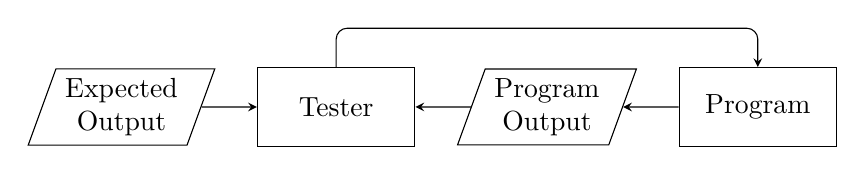
\begin{tikzpicture}
		\node (Tester)[process]{Tester};
		\node (Program Output)[io, right = 2em of Tester, align=center]{Program\\Output};
		\node (Program)[process, right = 2em of Program Output]{Program};
		\node (Expected Output)[io, left = 2em of Tester, align=center]{Expected\\Output};
		\draw [-stealth] (Expected Output) -- (Tester);
		\draw [-stealth] (Program Output) -- (Tester);
		\draw [-stealth] (Program) -- (Program Output);
		\draw [-stealth, rounded corners] (Tester.north) -- (0,1) -| (Program.north);
	\end{tikzpicture}
	\caption{External Program Side-effect Comparison Overview}
	\label{fig:autofigure1}
\end{figure}


\subsection{Internal Program Unit Testing}

\textit{Unit testing} is assumed to be the evaluation of \textit{individual discrete code components} within a tested program by comparing internal program state such as a function return value to a known expected state that has been pre-generated by a sample solution.

In internal program unit testing, the execution and collection of results from internal unit test cases can be used to determine whether expected behaviour has been achieved.

As a benefit, testing internal code components permits for finer control on the determination of program correctness by exposing internal functions instead of being reliant on observing side-effects. However, this benefit is traded off with the difficulty of unit testing more complex programs which may not be able the share the same unit testing framework throughout all components.

The interactions between the code tester and test program can be summarised in \autoref{fig:autofigure2}.

\begin{figure}[h]
	\centering
	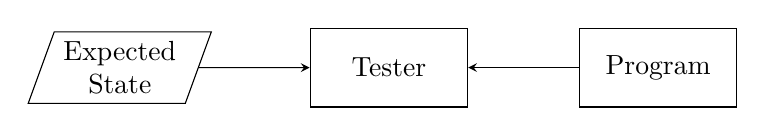
\begin{tikzpicture}
		\node (Tester)[process]{Tester};
		\node (Program)[process, right = 4em of Tester]{Program};
		\node (Expected Output)[io, left = 4em of Tester, align=center]{Expected\\State};
		\draw [-stealth] (Expected Output) -- (Tester);
		\draw [-stealth] (Program) -- (Tester);
	\end{tikzpicture}
	\caption{Internal Program Unit Testing Overview}
	\label{fig:autofigure2}
\end{figure}

\unchapter{3}{Related Works}

It is important to explore some existing work which could influence the design towards a chosen direction. In particular, the thesis will explore and evaluate \textit{autotest} - the current automated code testing tool used for introductory programming courses at UNSW \cite{Autotest}; \textit{check50} - another implementation of an automated code testing tool used in the CS50 introductory programming course at Harvard University \cite{check50}; and \textit{gtest} - a C++ unit testing framework used by Google and the programming community \cite{gtest}. Historic and minimally relevant implementations are also mentioned for completeness. 

\section{autotest}

As mentioned in Chapter 1, \textit{autotest} is a software package designed by Andrew Taylor to fulfil the purpose of an automatic code testing tool and has become the standard code testing tool for introductory programming courses at UNSW.

\subsection{Implementation \& Usage Overview}

\textit{autotest} is a tool that primarily follows the \textit{external program side-effect comparison} methodology to automatically determine the correctness of a tested program which can be seen in \autoref{fig:autotest1}. \textit{autotest} is written in Python but does expose some Bash shell and Perl script interfaces as a result of it's historical relation with the earlier script by Mei Cheng Whale.

\begin{figure}[h]
	\centering
	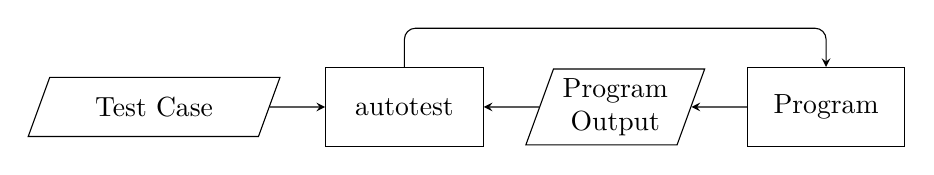
\begin{tikzpicture}
		\node (Tester)[process]{autotest};
		\node (Program Output)[io, right = 2em of Tester, align=center]{Program\\Output};
		\node (Program)[process, right = 2em of Program Output]{Program};
		\node (Expected Output)[io, left = 2em of Tester, align=center]{Test Case};
		\draw [-stealth] (Expected Output) -- (Tester);
		\draw [-stealth] (Program Output) -- (Tester);
		\draw [-stealth] (Program) -- (Program Output);
		\draw [-stealth, rounded corners] (Tester.north) -- (0,1) -| (Program.north);
	\end{tikzpicture}
	\caption{autotest High-level Architecture}
	\label{fig:autotest1}
\end{figure}

In terms of usage, \textit{autotest} provides a simplified interface to define multiple test cases with custom test parameters and environment in accordance with the needs of the user. In particular, the ability to set a time limit for each test case is valuable in handling cases where code may have an unintentional infinite loop, a common mistake made by beginners to programming.

\begin{figure}[h]
	\centering
	\begin{lstlisting}[linewidth=\linewidth]
files=is_prime.c
		
1 stdin="39" expected_stdout="39 is not prime\n"
2 stdin="42" expected_stdout="42 is not prime\n"
3 stdin="47" expected_stdout="47 is prime\n"
	\end{lstlisting}
	\caption{autotest Example Test Cases}
	\label{fig:autotest2}
\end{figure}

Files containing these test case specifications (\autoref{fig:autotest2}) can be saved to a directory and easily utilised by a wrapper script (\autoref{fig:autotest3}) which generalises and simplifies execution of the tool via abstraction of certain details from the intended end-user:

\begin{figure}[h]
	\centering
	\begin{lstlisting}[language=bash, breaklines=true, linewidth=\linewidth]
#!/bin/sh

parameters="
default_compilers = {'c' : [['gcc', '-Werror', '-std=gnu11', '-g', '-lm']]}
"

exec <path_to_autotest>/autotest.py -a <path_to_test_dir> --parameters "$parameters" "$@"
	\end{lstlisting}
	\caption{autotest Wrapper Script}
	\label{fig:autotest3}
\end{figure}

Upon execution of \textit{autotest} with a correct \textit{is\_prime.c}, the output shown in \autoref{fig:autotest4} is expected which informs the user that the provided test cases have passed. In this particular case, the tested program has successfully provided the expected output as defined by each of the test cases.

\begin{figure}[h]
	\centering
	\begin{lstlisting}[breaklines=true, linewidth=\linewidth]
gcc -Werror -std=gnu11 -g -lm -o is_prime is_prime.c
Test 1 (is_prime) - passed
Test 2 (is_prime) - passed
Test 3 (is_prime) - passed
3 tests passed 0 tests failed
	\end{lstlisting}
	\caption{autotest execution on correct program}
	\label{fig:autotest4}
\end{figure}

In the event that \textit{autotest} is executed with a flawed \textit{is\_prime.c}, \textit{autotest} will report to the user on the cause of the failure of a test case whether it is a mismatch in side-effects in the case of \autoref{fig:autotest5} or other cause such as compilation failure. Over the lifetime of \textit{autotest}, the unique situations that the tool can detect has increased which in turn provides users with additional targeted information and context.

This information is useful to both student and staff as it may be difficult to manually analyse the differences in larger amounts of side-effects created from more complex programs or program executions.  As such, it is one of the defining features that separates \textit{autotest} from other implementations.

\clearpage
\begin{figure}[h]
	\centering
	\begin{lstlisting}[breaklines=true, linewidth=\linewidth]
gcc -Werror -std=gnu11 -g -lm -o is_prime is_prime.c
Test 1 (is_prime) - passed
Test 2 (is_prime) - passed
Test 3 (is_prime) - failed (Incorrect output)
Your program produced this line of output:
47 is not prime

The correct 1 lines of output for this test were:
47 is prime

The difference between your output(-) and the correct output(+) is:
- 47 is not prime
?      ----

+ 47 is prime

The input for this test was:
47
You can reproduce this test by executing these commands:
gcc -Werror -std=gnu11 -g -lm -o is_prime is_prime.c
echo -n 47 | is_prime
2 tests passed 1 tests failed
	\end{lstlisting}
	\caption{autotest execution on incorrect program}
	\label{fig:autotest5}
\end{figure}

To ensure a test program's full compliance to a given specification with \textit{autotest}, sufficient test cases to cover all edge cases and standard execution will be required which can be a challenge depending on the complexity of the specification. However, checks on the creation of tests is out of scope for \textit{autotest}.

\subsection{Benefits}

Further analysis of \textit{autotest} and it's usage at UNSW can provide the following list of benefits for this thesis as an inspiration:
\begin{itemize}
	\item \textbf{\textit{autotest} has been proven to be mostly reliable at UNSW} - There have been undocumented reports of rare autotest crashes when being run in a distributed fashion but no documented reports could be found of the issue affecting administration of coding assessments within UNSW \cite{AutotestConversation}.
	\item \textbf{\textit{autotest} is able to support any programming language in which \textit{autotest} can detect and compare side-effects to determine program correctness} - This assists greatly in the usability of \textit{autotest} by courses that do not share an identical programming language as \textit{external program side-effect comparison} is a language-agnostic methodology.
	\item \textbf{\textit{autotest} exposes many parameters in the test case specification which allows users to have finer control over the test execution environment} - Some specifications that \textit{autotest} may want to test could require specialised testing environments for it's test cases.
	\item \textbf{\textit{autotest} has a side-effect comparison module that provides meaningful information on differences between actual and expected output in the event of a test failure} - This is one of the most defining components of \textit{autotest} in the assistance it provides to users.
\end{itemize} 

\subsection{Limitations}

Despite the benefits of \textit{autotest}, there are unfortunately some limitations that make \textit{autotest} unsuitable for continued use and have motivated this thesis:
\begin{itemize}
	\item \textbf{\textit{autotest} was not designed for long term maintainability and feature extensibility} - This is evident in the difficulty to change major components of \textit{autotest} without significant and difficult overhaul on large amounts of the code base as seen in the 2021 improvements by UNSW CSE.
	\item \textbf{\textit{autotest} has incorrect, outdated and insufficient documentation} - Although the mistakes in documentation are relatively minor such as typos, the insufficient and outdated information has been difficult to rectify. This has hindered the ability of contributors to understand how \textit{autotest} works at a deeper level and obstructed first-time users from utilising \textit{autotest} to it's fullest ability.
	\item \textbf{\textit{autotest} was not designed for security which is of concern in modern times} - When code testing foreign code as a result of marking, the current iteration of \textit{autotest} has no in-built protections against potentially malicious code such as deletion of system files (eg. ``\textit{sudo rm -rf /}"). This can be alleviated via external means such as limiting permissions for the user executing \textit{autotest} but this is only a short term solution.
	\item \textbf{\textit{autotest} has performance issues as a result of it's original design} - \textit{autotest} was not originally intended to be utilised at the scale as it is today. As such, it's most significant performance issue is the single-threaded nature of \textit{autotest} where there is no accepted implementation to execute unrelated tests in parallel \cite{AutotestParallelisation}.
\end{itemize}

\section{check50}

\textit{check50} is a software package designed by Chad Sharp and others at Harvard University to fulfil the purpose of an automatic code testing tool. Similar to \textit{auotest}, \textit{check50} which was first introduced in 2012 has also become the standard code testing tool for the \textit{CS50: Introduction to Computer Science} course at Harvard University.

\subsection{Implementation \& Usage Overview}

\textit{check50} is a tool that primarily follows the \textit{external program side-effect comparison} to automatically determine the correctness of a tested program which can be seen in \autoref{fig:check501}. \textit{check50} is written in Python and receives active maintenance and development efforts via a private repository \cite{check50Github}.

\begin{figure}[h]
	\centering
	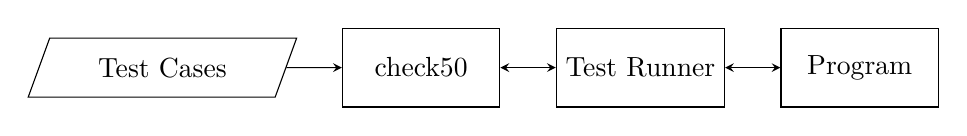
\begin{tikzpicture}
		\node (Tester)[process]{check50};
		\node (Tests)[io, left = 2em of Tester, align=center]{Test Cases};
		\node (Test Runner)[process, right = 2em of Tester]{Test Runner};
		\node (Program)[process, right = 2em of Test Runner]{Program};
		\draw [-stealth] (Tests) -- (Tester);
		\draw [stealth-stealth] (Tester) -- (Test Runner);
		\draw [stealth-stealth] (Test Runner) -- (Program);
	\end{tikzpicture}
	\caption{check50 High-level Architecture}
	\label{fig:check501}
\end{figure}

In terms of usage, \textit{check50} provides a simple framework for defining the test cases as well as an easy-to-use API that abstracts common tasks such as compiling and running away from the user. In line with the goals of \textit{check50}, the creation of test cases known as ``checks" is simplified into a chain of functions in Python similar to that seen in functional languages such as Haskell. YAML checks can also be defined but are converted into Python automatically on execution of these checks by \textit{check50}.

\begin{figure}[h]
	\centering
	\begin{lstlisting}[language=python, breaklines=true, linewidth=\linewidth]
import check50
import check50.c

@check50.check()
def exists():
"""hello.c exists"""
check50.exists("hello.c")

@check50.check(exists)
def compiles():
"""hello.c compiles"""
check50.c.compile("hello.c", lcs50=True)

@check50.check(compiles)
def emma():
"""responds to name Emma"""
check50.run("./hello").stdin("Emma").stdout("Emma").exit()
	\end{lstlisting}
	\caption{check50 Example Test Cases (Checks)}
	\label{fig:check502}
\end{figure}

Files containing these checks (\autoref{fig:check502}) can be saved to a directory locally or online to be executed as a ``slug" which is the relative path to the directory containing checks. Since \textit{check50} is officially recommended to be installed as a pip package, execution of \textit{check50} on a slug is relatively simple as seen in \autoref{fig:check503} \cite{check50Docs}. It is also observed that upon execution of \textit{check50} with a correct \textit{hello.c}, the tool reports to the user that the provided checks have passed. In this particular case, the tested program has successfully completed all checks as defined.

\begin{figure}[h]
	\centering
	\begin{lstlisting}[breaklines=true, linewidth=\linewidth]
$ check50 <path_to_example_checks>
:) hello.c exists
:) hello.c compiles
:) responds to name Emma
	\end{lstlisting}
	\caption{check50 execution on correct program}
	\label{fig:check503}
\end{figure}

In the event \textit{check50} is executed with a flawed \textit{hello.c}, \textit{check50} will report to the user on the failure of a test case whether it is a mismatch in side-effects in the case of \autoref{fig:check504} or other cause such as compilation failure. \textit{check50} supports the provision of a hint string in the failure of the test case but this must be manually set by the test writer and may potentially distract from the issue if the hint is not appropriate.

\clearpage
\begin{figure}[h]
	\centering
	\begin{lstlisting}[breaklines=true, linewidth=\linewidth]
$ check50 <path_to_example_checks>
:) hello.c exists
:) hello.c compiles
:( responds to name Emma
	expected "Emma\n", not "emma\n"
	<hint_string_here>
	\end{lstlisting}
	\caption{check50 execution on incorrect program}
	\label{fig:check504}
\end{figure}

Similarly to \textit{autotest}, to ensure a test program's full compliance to a given specification with \textit{check50}, sufficient checks to cover all edge cases and standard execution will be required which can be a challenge depending on the complexity of the specification. However, evaluation of checks for a specification is out of scope for \textit{check50}. 

\subsection{Benefits}

Further analysis of \textit{check50} can provide the following list of benefits for this thesis as an inspiration:
\begin{itemize}
	\item \textbf{\textit{check50} test cases or checks are very easy to create} - There are many examples of checks that are available publicly and the difficulty of creating checks for basic programs is significantly lower than \textit{autotest} \cite{check50Examples}.
	\item \textbf{\textit{check50} is theoretically able to support any programming language} - This assists greatly in the usability of \textit{check50} by courses that do not share an identical programming language as \textit{check50} is declared to be theoretically language-agnostic assuming the user implements the necessary tooling for the language such as the framework and API.
	\item \textbf{\textit{check50} maintains extensive and up-to-date documentation} - This is a significant benefit as the extensive documentation supports users in their understanding on the more confusing components of \textit{check50} which has made usage of the tool and code contributions much easier.
	\item \textbf{\textit{check50} has a module that converts \textit{check50} output into a HTML page that improves readability of results for users who may find terminal output difficult to read} - This is one of the most defining components of \textit{check50} in the benefit of this thesis as it improves accessibility of the tool to students who may have difficulties with sight.
	\item \textbf{\textit{check50} implements containerisation of checks as a security measure against potentially malicious code and can be configured to run both remotely or locally} - This is an important feature that offers significant long term advantages such as infrastructure safety and scalability by keeping infrastructure secure and permitting users to run checks locally respectively. As such, it is a significant advantage that \textit{check50} has over \textit{autotest}.
	\item \textbf{\textit{check50} supports concurrent execution of tests} - Concurrent execution of unrelated tests takes advantage of the full resources offered by a computer to evaluate all checks in a minimal amount of time which increases performance and efficiency. As an added benefit, \textit{check50} checks have the ability to define an execution order or dependency graph which ensures that certain checks such as tests on the existence of certain files and compilation are executed first before checks that depend on them. 
\end{itemize} 

\subsection{Limitations}

Despite the benefits of \textit{check50}, there are unfortunately some limitations that make \textit{check50} nonviable for immediate use and have motivated this thesis:

Assume \textit{harnessing} to be programs and tooling that is specifically created for the purposes of creating side-effects or other usable information from programs that do not generate such information alone. An example of \textit{harnessing} would be a test program that outputs the return value of a function that is not exposed to the user under normal operating conditions. 

\begin{itemize}
	\item \textbf{\textit{check50} has an emphasis on the easy creation of tests which has resulted in larger amounts of abstractions and complicated the execution of complex programs} - This could be mitigated by harnessing the complex programs to work with \textit{check50} but this is a short term solution and could involve significant work by the user to implement.
	\item \textbf{\textit{check50} has no official support for languages outside of C, Python and Python Flask} - Although support can be implemented for different languages, there is likely a non-trivial amount of work that is necessary with no guarantee that the implementation by the user will be correct. This could once again be mitigated by harnessing but the same flaw of being a short term solution and potentially requiring significant work remains.
\end{itemize}

\clearpage
\section{gtest}

\textit{gtest} is a testing and mocking framework originally designed by Google to fulfil the purpose of testing Google's internal C++ projects. \textit{gtest} has since been released to the public in 2008 and has become one of the most popular C++ testing tools that is publicly available as open source software.

\subsection{Implementation \& Usage Overview}

\textit{gtest} is a tool that primarily follows the \textit{internal program unit testing} methodology to automatically determine the correctness of a tested program which can be seen in \autoref{fig:gtest1}. It could theoretically support \textit{external program side-effect comparison} but it would require significant harnessing efforts that may not carry over for different specifications. \textit{gtest} is written in C++ and receives active maintenance and development efforts by both Google and the open source software community.

\begin{figure}[h]
	\centering
	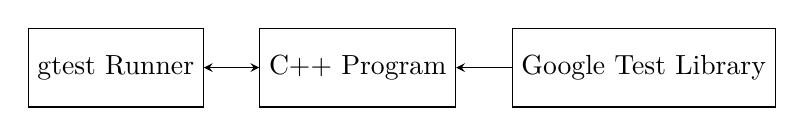
\begin{tikzpicture}
		\node (Tester)[process]{gtest Runner};
		\node (Program)[process, right = 2em of Tester]{C++ Program};
		\node (Tooling)[process, right = 2em of Program]{Google Test Library};
		\draw [stealth-stealth] (Tester) -- (Program);
		\draw [-stealth] (Tooling) -- (Program);
	\end{tikzpicture}
	\caption{gtest High-level Architecture}
	\label{fig:gtest1}
\end{figure}

In terms of usage, \textit{gtest} approaches defining of test cases in a unique way in comparison to \textit{autotest} or \textit{check50}. In particular, test cases are able to specifically target internal components of a tested program such as functions without harnessing unlike \textit{autotest} and \textit{check50} that can only target the tested program as a whole without the use of harnessing.

\begin{figure}[h]
	\centering
	\begin{lstlisting}[language=c++, breaklines=true, linewidth=\linewidth]
// test.h
#include "is_prime.h"
#include <gtest/gtest.h>

TEST(IsPrimeTest, Positive) {
	EXPECT_FALSE(IsPrime(4));
	EXPECT_TRUE(IsPrime(5));
	EXPECT_FALSE(IsPrime(6));
	EXPECT_TRUE(IsPrime(23));
}
	\end{lstlisting}
	\caption{gtest Example Test Cases}
	\label{fig:gtest2}
\end{figure}

Files containing these test case specifications (\autoref{fig:gtest2}) can be saved to a directory and executed via a \textit{gtest} runner which will automatically collect all tests from linked files when compiled and run (\autoref{fig:gtest3}):

\begin{figure}[h]
	\centering
	\begin{lstlisting}[language=c++, breaklines=true, linewidth=\linewidth]
// main_test.cc
#include <gtest/gtest.h>

#include "test.h"
// link all other test specification files here

int main(int argc, char **argv) {
	testing::InitGoogleTest(&argc, argv);
	return RUN_ALL_TESTS();
}
	\end{lstlisting}
	\caption{gtest runner Source Code}
	\label{fig:gtest3}
\end{figure}

\begin{figure}[h]
	\centering
	\begin{lstlisting}[breaklines=true, linewidth=\linewidth]
$ ./main_test
[==========] Running 1 test from 1 test suite.
[----------] Global test environment set-up.
[----------] 1 test from IsPrimeTest
[ RUN      ] IsPrimeTest.Positive
[       OK ] IsPrimeTest.Positive (0 ms)
[----------] 1 test from IsPrimeTest (0 ms total)

[----------] Global test environment tear-down
[==========] 1 test from 1 test suite ran. (0 ms total)
[  PASSED  ] 1 test.
	\end{lstlisting}
	\caption{gtest runner execution on correct program}
	\label{fig:gtest4}
\end{figure}

\begin{figure}[h]
	\centering
	\begin{lstlisting}[breaklines=true, linewidth=\linewidth]
$ ./main_test
[==========] Running 1 test from 1 test suite.
[----------] Global test environment set-up.
[----------] 1 test from IsPrimeTest
[ RUN      ] IsPrimeTest.Positive
main_test.cc:17: Failure
Value of: IsPrime(23)
Actual: false
Expected: true
[  FAILED  ] IsPrimeTest.Positive (0 ms)
[----------] 1 test from IsPrimeTest (0 ms total)

[----------] Global test environment tear-down
[==========] 1 test from 1 test suite ran. (0 ms total)
[  PASSED  ] 0 tests.
[  FAILED  ] 1 test, listed below:
[  FAILED  ] IsPrimeTest.Positive

1 FAILED TEST
	\end{lstlisting}
	\caption{gtest runner execution on incorrect program}
	\label{fig:gtest5}
\end{figure}

\clearpage
Upon execution of the \textit{gtest runner} with a correct \textit{is\_prime.cc} and \textit{is\_prime.h}, the output shown in \autoref{fig:gtest4} is expected which informs the user that the provided test cases have passed. In this particular case, all assertions of the \textit{isPrimeTest} test case have passed.

In the event \textit{gtest runner} is executed with a flawed \textit{is\_prime.cc} or \textit{is\_prime.h}, \textit{gtest} will report to the user on the cause of the failure of a test case such as a deviation from expected behaviour as seen in \autoref{fig:gtest5}.

To ensure a test program's full compliance to a given specification with \textit{gtest}, sufficient test cases to cover all edge cases and standard execution will be required which can be a challenge depending on the complexity of the specification. However, checks on the creation of tests is out of scope for \textit{gtest}.

\subsection{Benefits}

Further analysis of \textit{gtest} can provide the following list of benefits for this thesis as an inspiration:
\begin{itemize}
	\item \textbf{\textit{gtest} maintains extensive and up-to-date documentation with a large community of users} - This is a significant benefit as \textit{gtest} as a whole can be perceived as complicated and confusing but many community made tutorials and guides exist on the internet to solve most issues.
	\item \textbf{\textit{gtest} supports concurrent execution of tests} - Concurrent execution of unrelated tests takes advantage of the full resources offered by a computer to evaluate all test cases in a minimal amount of time which increases performance and efficiency. However, \textit{gtest} offers no methods to guarantee that tests will be executed in a certain order unlike \textit{check50}. 
\end{itemize} 

\subsection{Limitations}

Despite the benefits of \textit{gtest}, there are unfortunately some limitations that make \textit{gtest} unsuitable for use:
\begin{itemize}
	\item \textbf{\textit{gtest} is not designed to test whole programs and can have trouble detecting side-effects such as the existence of files without significant harnessing} - This is expected for software that implements \textit{internal program unit testing} as a methodology but still remains a significant limitation of \textit{gtest} for use as an automated code testing tool.
	\item \textbf{\textit{gtest} does not sufficiently support test execution environment configuration easily} - \textit{Internal program unit testing} frameworks are not expected to manage an external test environment but the difficulty and lack of configuration within \textit{gtest} could prevent the testing of programs that may rely on a specialised environment.
	\item \textbf{\textit{gtest} is generally difficult to use as an automated code testing tool} - \textit{gtest} is difficult to configure and utilise for most users and far better tools such as \textit{autotest} and \textit{check50} exist for a baseline design.
\end{itemize}

\section{Other \& Historic Works}
See these other and historic works that have had minimal but relevant impact on this thesis as an exploration on the progression of each aforementioned automated code testing methodology throughout history: \textbf{JUnit} (Internal Program Unit Testing) \cite{junit}, \textbf{BAGS} (Primitive External Program Side-effect Comparison) \cite{bags}, \textbf{Kassandra} (External Program Side-effect Comparison) \cite{kassandra} and \textbf{TRY} (External Program Side-effect Comparison) \cite{try}. 

\unchapter{4}{Approach}

\section{Requirements}

The initial problem statement of introducing a replacement automated code testing tool is quite broad, and the required design will depend highly on the chosen automated testing approach. In particular, it would be impossible to have one solution that will immediately satisfy the demands of all users.

Therefore it is important to lay out the desired requirements and design goals for an ideal solution before choosing a proposed approach for the implementation.

\subsection{Design Goals}

In accordance with the thesis aim, the design goals for the project will emphasise the following properties:

\begin{itemize}
	\item \textbf{Accessibility} - The design should allow new users to easily integrate this automated code testing tool into their coding assessments.
	\item \textbf{Familiarity} - Existing users of \textit{autotest} should not observe the proposed solution and it's usage to be completely independent of the former.
	\item \textbf{Performance \& Efficiency} - The proposed implementation should be observed to have comparable if not better performance than the existing \textit{autotest}. Benchmarking of \textit{autotest} and the proposed implementation will be performed to verify this goal.
	\item \textbf{Maintainability} - The design should be adequately documented and support an ease of maintainability and possible extension of features via the appropriate architectural decisions.
\end{itemize}

In addition to the aforementioned, the thesis will also emphasise the following but at a lower priority due to time constraint limitations:

\begin{itemize}
	\item \textbf{Security} - The design should implement or consider the addition of security as it has been a concern for various implementations of an \textit{automated code testing tool} in the protection of user hardware against potentially malicious code.
\end{itemize}

It is noted that most of these goals are qualitative and can not be quantitatively measured outside of reader observation. The thesis will attempt to quantify these goals within the properties of each proposed design approach but it will still be dependent on the reader's interpretation.

\section{Design}

From the evaluation of the related works, the thesis evaluates two potential design approaches to the solution that fulfils the design goals outlined above, one of these two approaches is then chosen for the project. Implementation details for each design approach are important but defining a ``target" architecture design is considered to be of greater importance as it cannot be easily changed once development begins.

\subsection{check50 Approach}

In this approach, the architectural design will be similar to that of \textit{check50} as shown in \autoref{fig:approach1-1} including the design for definition of test cases and as such, the methodology to determine correctness of a tested program will be \textit{external program side-effect comparison}.

\begin{figure}[h]
	\centering
	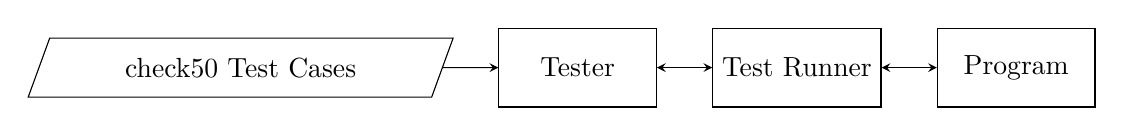
\begin{tikzpicture}
		\node (Tester)[process]{Tester};
		\node (Tests)[io, left = 2em of Tester, align=center]{check50 Test Cases};
		\node (Test Runner)[process, right = 2em of Tester]{Test Runner};
		\node (Program)[process, right = 2em of Test Runner]{Program};
		\draw [-stealth] (Tests) -- (Tester);
		\draw [stealth-stealth] (Tester) -- (Test Runner);
		\draw [stealth-stealth] (Test Runner) -- (Program);
	\end{tikzpicture}
	\caption{check50 Approach - High-level Architecture}
	\label{fig:approach1-1}
\end{figure}

This approach allows the project to utilise \textit{check50} as a ``baseline" for both performance and correctness testing of the solution which will aid in the development process by being a reference solution that can be compared with.

To further develop the approach, a solution implementing this approach would work like so (at a high level):
\begin{enumerate}
	\item The \textit{Tester} will read in the appropriate \textit{test cases} and any other relevant information to parse into individual test cases with the relevant parameters set (timeout period, test input, expected output etc).
	\item The \textit{Tester} will ``spin up"/initialise a configured amount of \textit{Test Runner} processes which will each individually consume a test case for independent execution.
	\item When the \textit{Test Runner} completes execution of a test which may involve an external \textit{Program}, the \textit{Test Runner} will return it's result back to the \textit{Tester} and consume another test for execution if one exists. If no more tests exist, the waiting \textit{Test Runner} will ``spin down"/shut down.
	\item Throughout steps 2 and 3, the \textit{Tester} will report to the user on test execution progress but once all tests results have been gathered, a report will be generated for the user on test successes and failures.
\end{enumerate}

\subsection{autotest Approach}

In this approach, the architecture is similar to the \textit{check50 Approach} in Section 4.2.1 but with the distinct change that the design of the test case definitions will be that of the existing \textit{autotest}.

\begin{figure}[h]
	\centering
	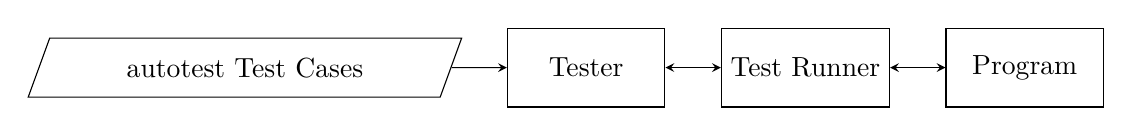
\begin{tikzpicture}
		\node (Tester)[process]{Tester};
		\node (Tests)[io, left = 2em of Tester, align=center]{autotest Test Cases};
		\node (Test Runner)[process, right = 2em of Tester]{Test Runner};
		\node (Program)[process, right = 2em of Test Runner]{Program};
		\draw [-stealth] (Tests) -- (Tester);
		\draw [stealth-stealth] (Tester) -- (Test Runner);
		\draw [stealth-stealth] (Test Runner) -- (Program);
	\end{tikzpicture}
	\caption{autotest Approach - High-level Architecture}
	\label{fig:approach2-1}
\end{figure}

The original architecture of \textit{autotest} has been abandoned in this approach as the \textit{check50} architecture is more suitable to the aforementioned design goals.

Thus, the solution implementing this approach will be identical to the \textit{check50 approach} and has been omitted as it is available in Section 4.2.1.

\subsection{Chosen Approach}

Evaluation of each approach was made by considering fulfilment of the design goals aforementioned above. \autoref{tab:table2} lists if each approach satisfies each design requirement.

\begin{table}[h]
	\centering
	\begin{tabular}{lll}
		\toprule
		\textbf{Requirement} & \textbf{check50 Approach} & \textbf{autotest Approach} \\
		\midrule
		Accessibility    & Yes (by design) & Yes (by design) \\
		Familiarity      & No  & Yes \\
		Performance \& Efficiency & Unknown & Unknown \\
		Maintainability  & Yes (Technical Debt Management) & Yes (Technical Debt Management) \\
		Security 		 & Planned & Planned \\
		\bottomrule
	\end{tabular}
	\caption{Evaluation of the \textit{check50} and \textit{autotest} approach against the stated requirements}
	\label{tab:table2}
\end{table}

As seen from \autoref{tab:table2}, neither approach completely matches the requirements laid out, however the \textit{autotest approach} is close and will serve as an appropriate start for the project over the alternative.

It is noted that some components of the test case definition design and backend design of \textit{check50} could be considered to be superior to that of \textit{autotest}. As these features are implementations details and are not greatly affected in respect to the chosen architecture, decisions on whether these features will be included in the solution can be deferred to a later time in the development period.

It is also noted that the chosen approach has changed since Seminar A due to the inclusion of security in the design goals which had been justified by Seminar A feedback \cite{AutotestConversation}. Although security is a low priority goal, this was sufficient reason to modify the proposed architecture of the \textit{autotest approach}.

\unchapter{5}{Preliminary Work \& Plan}

\section{Preliminary Work}

\subsection{Usage Survey}

As a result of feedback during the Thesis A Seminar, a survey listing the following questions is being distributed to the various course administrators of introductory programming courses at UNSW (COMP1511, COMP1521, COMP1531 and COMP2521):
\begin{enumerate}
	\item Do you use autotest in the courses you administrate? If so, for what purpose (marking labs and assignments etc)?
	\item Do you believe there are issues/weaknesses with autotest? If so, could you describe them?
	\item Do you believe there are strengths with autotest? If so, could you describe them?
	\item How much change would be acceptable with the current autotest before you consider remaining with the original version?
	\item Would you be interested in being kept up-to-date on a thesis project updating and replacing autotest? (This is not mandatory and participation is optional although it will be of great help to the project)
\end{enumerate}

The results of these surveys will be collected and used to make informed decisions within the Design Document. In the event of interest by the course administrator, the course administrator will be regularly apprised of details within the Design Document to gather feedback which can be used to justify changes or a lack of change.

\subsection{Design Document}

The design document will contain all implementation details of the thesis project and will be the single source of truth for the project. Minimal work has been done on this document but it is expected to be populated rapidly in the near future.

\section{Thesis Project Plan}

This is the intended schedule for Thesis B:
\begin{itemize}
	\item \textit{Week 1: Initial finalisation of Design Document.} This will involve:
	\begin{itemize}
		\item Collection of feedback from supervisor, assessor and all relevant personnel.
		\item Final adjustments for the initial design document.
	\end{itemize}
	\item \textit{Weeks 2-3: Core Tester/Main Module.} This will involve implementation of the core tester/main module in accordance with the design document and any appropriate adjustments.
	\item \textit{Weeks 3-6: Core Testcase Parser Module.} This will involve:
	\begin{itemize}
		\item Implementation of core testcase parser module in accordance with the design document.
		\item Adjustments made to the design document in respect to changing requirements/challenges.
		\item Performance and Correctness testing run on testcase parser and results recorded.
	\end{itemize}
	\item \textit{Weeks 7-11: Core Testcase Runner Module.} This will involve:
	\begin{itemize}
		\item Implementation of core testcase runner module in accordance with the design document.
		\item Adjustments made to the design document in respect to changing requirements/challenges.
		\item Performance and Correctness testing run on testcase runner and results recorded.
	\end{itemize}
	\item \textit{Week 11: Testing with Core Tester/Main Module.} This will involve correctness testing of the core tester/main module.
\end{itemize}

Then for Thesis C:
\begin{itemize}
	\item \textit{Weeks 1-4: Core Testcase Program Correctness Module.} This will involve:
	\begin{itemize}
		\item Implementation of core testcase program correctness module in accordance with the design document.
		\item Adjustments made to the design document in respect to changing requirements/challenges.
		\item Performance and Correctness testing run on testcase program correctness module and results recorded.
	\end{itemize}
	\item \textit{Weeks 5-6: MVP Milestone \& Testing for autotest replacement.} This will involve:
	\begin{itemize}
		\item Designation of thesis project as having reached the Minimal Viable Product milestone.
		\item Performance and Correctness testing run on thesis project and results recorded.
		\item Replacement or parallelisation (for deferred cut-over) of existing autotest with the thesis project.
	\end{itemize}
	\item \textit{Weeks 7-8: Implementation of extensions and any other tasks.} This will involve:
	\begin{itemize}
		\item Implementation of any extensions that have been documented in the design document.
		\item Any additional tasks that have taken longer than expected.
		\item Final adjustments before Thesis C demonstration.
		\item Benchmarking of the final thesis project before Thesis C demonstration.
	\end{itemize}
	\item \textit{Weeks 9-11: Write final Thesis C report.}
\end{itemize}

\unchapter{6}{Conclusion}

The above thesis outlines the possible methodologies of automated code testing, it's usage in relevant existing works and proposes a design approach for achieving the aim of this thesis which is to create an automated code testing tool in respect to the given design goals in Section 4.1.
Preliminary work has been completed and a plan for the implementation of the proposed design has been provided to demonstrate the feasibility of this thesis.

% 99 here is used as a placeholder for the number of digits. If you for some reason have over 99 references change it to 999.
\begin{thebibliography}{99}
	
\bibitem[1]{Autotest}
Andrew Taylor, ‘autotest’, URL: \url{https://github.com/COMP1511UNSW/autotest}

\bibitem[2]{TechnicalDebtConcept}
Ward Cunningham, ‘The WyCash Portfolio Management System’ in \textit{Addendum to the Proceedings on Object-Oriented Programming Systems, Languages, and Applications (addendum)} (ACM, 1992) 29

\bibitem[3]{TechnicalDebt}
Tom Edith, Aybüke Aurum and Richard Vidgen, ‘An Exploration of Technical Debt’ (2013) 86(6) \textit{The Journal of systems and software 1498}

\bibitem[4]{AutotestIssues}
Andrew Taylor et al., ‘autotest issues’, URL: \url{https://github.com/COMP1511UNSW/autotest/issues}

\bibitem[5]{TechnicalDebtManagement}
Eric Allman, ‘Managing Technical Debt’ (2012) 55(5) \textit{Communications of the ACM} 50

\bibitem[6]{ManualProblem}
David Jackson, ‘Using Software Tools to Automate the Assessment of Student Programs’ (1991) 17(2) \textit{Computers and education} 133

\bibitem[7]{AutomatedFirst}
Jack Hollingsworth, ‘Automatic Graders for Programming Classes’ (1960) 3(10) \textit{Communications of the ACM 528}

\bibitem[8]{check50}
Chad Sharp et al, ‘An Open-Source, API-Based Framework for Assessing the Correctness of Code in CS50’ in \textit{Proceedings of the 2020 ACM Conference on Innovation and Technology in Computer Science Education} (ACM, 2020) 487

\bibitem[9]{gtest}
Google, ‘GoogleTest’, URL: \url{https://github.com/google/googletest}

\bibitem[10]{check50Github}
Chad Sharp et al, ‘check50’, URL: \url{https://github.com/cs50/check50}

\bibitem[11]{AutotestConversation}
Andrew Taylor et al, Conversation at conclusion of Thesis A seminar for ‘A Testing Tool for Introductory Programming Courses’, 22 April

\bibitem[12]{check50Docs}
Chad Sharp et al, ‘check50 Documentation’, URL: \url{https://cs50.readthedocs.io/projects/check50/en/latest/}

\bibitem[13]{check50Examples}
Chad Sharp et al, ‘CS50 Problem Exercise Repository’, URL: \url{https://github.com/cs50/problems}

\bibitem[14]{AutotestParallelisation}
Kyu-Sang Kim, ‘autotest test case execution parallelisation proposal’, URL: \url{https://github.com/COMP1511UNSW/autotest/pull/28}

\bibitem[15]{junit}
Kent Beck et al, ‘JUnit’, URL: \url{https://github.com/junit-team/junit5}

\bibitem[16]{bags}
J Hext and J Winings, ‘An Automatic Grading Scheme for Simple Programming Exercises’ (1969) 12(5) \textit{Communications of the ACM} 272

\bibitem[17]{kassandra}
Urs von Matt, ‘Kassandra’ (1994) 22(1) \textit{SIGCUE bulletin} 26

\bibitem[18]{try}
Kenneth A Reek, ‘The TRY System -or- How to Avoid Testing Student Programs’ (1989) 21(1) \textit{ACM SIGCSE Bulletin} 112

\end{thebibliography}

\end{document}
